\chapter{Log}
\section{9/24/2023}
Braden created a new PROS project for team ATUM. This project will contain the
code for both robots. Braden began researching unit testing solutions and found
examples from OkapiLib using Google Test \cite{bib:okapilib} and from team
7842F/B's Change Up code using doctest \cite{bib:lib7842}. By being able to test
units of our code without a robot, we will be able to produce software with
fewer bugs.
\section{9/25/2023}
After much testing, Braden managed to get testing using doctest working locally
and then in a test repository via GitHub actions. The workflow takes much
inspiration from OkapiLib's implementation, while the actual Makefile is
indebted to 7842F's examples. Now the unit testing should be further stress
tested.
\section{9/26/2023}
Braden got GitHub Actions to automate the unit testing process and performed
further testing. The code has been separated into an API and implementation
section. The API section will contain references to only abstract devices (i.e.
classes that represent real-world devices, but don't contain references to the
VEX SDK) while the implementation contains references to real devices. It's
split up like this to facilitate doctest. \par Additionally, the Makefile for
the PROS project was updated to allow C++20 features.
Refer to the image below:
\begin{figure}
    \centering
    
\includegraphics[width=0.5\linewidth]{images/member photos/walter.png}
    
\end{figure}
\section{9/27/2023}
Braden added Valgrind for memory leak detection and automated the process
through GitHub Actions. The next immediate goal is test coverage statistics
collection and reporting.
\section{10/3/2023}
Braden walked Darrius through working with the notebook and code repositories.
\section{10/12/2023}
Braden set up two more scripts to run both clang-format and Cppcheck.
Clang-format is ran on each file in the repository and applies formatting rules.
Cppcheck looks for common mistakes with C++ code in all files in the repository.
A yaml file was also made to allow GitHub Actions to format the code upon
pushing. Collection of test coverage statistics are currently abandoned (but may
be tried again later).
\section{10/19/2023}
Braden added a library\cite{bib:unitslib} for performing dimensional analysis
(using physical units like meters, feet, and so on). This will be helpful for
disambiguating units used throughout the project. This specific library was
chosen because it is header-only (and, thus, easier to add) and has seen fairly
popular usage. \par Braden and Darrius also discussed how to use bang-bang and
PID to control systems on the robot as well as the scripts for workflow. Braden
created an interface class for controllers and got started on a bang-bang class.
Darrius began work on a PID class.
\section{11/2/2023}
Braden added a temporary version of the driver control program for testing
purposes Braden added a library\cite{bib:jsonlib} for read and writing JSON
files. Using an SD card, this will be used to allow configuration of ports and
other settings on-the-fly. Braden began work on this by experimenting with file
creation and reading from the SD card.
\section{11/16/2023}
Darrius has begun looking through learncpp\cite{bib:learncpp} to gain more
familiarity with the language. Braden began work on a dynamic current limiting
system. The brain can only provide 20A at a time to motors and each motor can
only take in a maximum of 2.5A. Thus, with 20A / 8 motors gives 2.5A the max
allocation per each motor and 20A / 11 motors gives 1.81A per each motor (about
70\% of the max possible). This is how current limiting is naively done in VEX,
but PROS gives the option to change the current limit on each motor. While this
could be done at the start of the match, say, for instance:
\begin{itemize}
    \item Six Drive Motors: 2.5A
    \item Two Flywheel Motors: 1.5A
    \item Three Other Motors: 0.66A
\end{itemize}
As $6 \cdot 2.5A + 2 \cdot 1.5A + 3 \cdot 0.66A \thickapprox  20A $, this would
work, but there may be times when the drive motors aren't drawing 2.5A (most of
the time, in fact). At these times, the limit on the other subsystems is
wasteful. For this reason, a system that dynamically adjusts the current limits
would be preferred. Braden also continued working on the SD card settings
system, managing to serialize a struct.
\section{1/11/2024}
Having paused work during the winter break, Braden decided the first priority
software-wise should be to improve unit test speed. CMake is now being used to
help generate the Makefile for testing and has been demonstrated to greatly
improve test speed. Now unit testing can be employed as intended without
impeding development.
\section{1/21/2024}
Due to some issues with building the PROS project, Braden decoupled testing from
the main source files into its own folder. Braden also worked on formalizing the
settings manager. A jumper cable has been added to the 15" bot in order to
distinguish it. This allows us to upload the same project to both bots and have
each configure themselves separately.
\section{1/30/2024}
Braden has spent the last two weeks reading several resources regarding Kalman
filters in order to develop a robust system to combine information from the
several sensors on the robot recording position. Within the next few days,
Braden will put together an outline of an Unscented Kalman Filter to combine
information from drive predictions, odometry, GPS readings, and the IMU. Before
that, a model must be designed for the robot's drive in order to make
predictions. So, today, Braden developed a simulation of the robot in Python
using Pygame\cite{bib:pygame}. The simulation is currently controlled by a V5
controller, but can be fed in input automatically to test other features, like
path following. The model the simulation uses near-certainly isn't very accurate
at the moment, as certain parameters (such as mass) are currently guesses;
though, the motor parameters were given by several motor statistics helpfully
provided by BLRS\cite{bib:blrsmotors}. The model takes much inspiration from
Controls Engineering in FRC\cite{bib:controlinfrc}. For learning about Kalman
filters, Kalman and Bayesian Filters in Python\cite{bib:kalmaninpython}.
Additionally, Braden added formatting to code in the notebook, seen below.
\begin{lstlisting}[language=Python]
    print("Hello world! Here's a number: " + 123); # This is a comment.
\end{lstlisting}
\section{2/4/2024}
Darrius has begun to research various autonomous routines from both university
and high school level. Darrius will produce plans for several autonomous
routines and programming skills over the next week or so. Braden has spent the
weekend outlining how a UKF would work on the robots using the developed Python
simulation. The proposed system would combine data from odometers, IMUs, the GPS
sensor, and a physics model to provide a better estimate of position. Braden has
also begun work on a trajectory planner and a controller to follow said plan.
This work has been guided by several resources spanning the BLRS
wiki\cite{bib:blrsramsete}, WPILib\cite{bib:wpiramsete}, and Control Theory in
FRC\cite{bib:controlinfrc}. In order to follow the references given by the
RAMSETE controller, a PID-ff controller was also developed. This controller
takes much inspiration from a series of blogs by Brett
Beauregard\cite{bib:pidimprove}.
\section{2/6/2024}
Braden has begun translating the progress made in the Python simulation to the
actual C++ project. This involves fleshing out several subsystems currently on
the robot, to even have the framework to support software solutions like Kalman
filters or RAMSETE. The prototype of the logger was the first brought over and
documented. Followed by a class for drives. The idea is that a driving strategy
will take in a drive as a parameter in order to perform some specific movement.
This would allow us to decouple different movement strategies (like moving to a
point, RAMSETE, pure pursuit, etcetera) from the drive itself. Additionally, a
wrapper for the PROS implementation of tasks was created to allow objects to
have "parallel behavior" (derive from said class and override a task function
that will be run as a separate process).
\section{2/7/2024}
Darrius worked on a pseudocode version and mapping of our planned autonomous
routines for matches and skills. Braden further documented the remote wrapper
and tested the current code on the robots. Additionally, Darrius added code to
turn the LEDs we have on each bot on.
\section{2/8/2024}
Braden further tested printing to the remotes and discovered an issue with
deadlocking which was fixed.
\section{2/10/2024}
Braden added a wrapper class around the GPS sensor implementation PROS provides.
This is because the standard GPS class does not deal with the units library we
are employing, as well as possessing an undesirable interface; for instance,
there is currently no command provided to check if the GPS sensor is calibrating
or not (our implementation has to read the errno PROS sets).
\section{2/11/2024}
Braden added a wrapper class around the IMU to support using several IMUs as if
they were one unit. Additionally, the class performs integration to estimate our
position on the field. It won't be particularly accurate for that purpose (in
fact, it is famously awful for tracking position), but will be integrated into
our UKF alongside other sensors to get a better estimate of our position
overall. Braden also added an odometer class to wrap around the PROS ADI
encoders to account for difference between standard VEX encoders and our
AMT102s. It also returns distance traveled since last checked (based on the
wheel circumference given), which is useful for odometry. Braden also added an
odometry class that implements two parallel encoder odometry. While quite
different from their implementation, it is still valuable to credit Pilons for
their classic document going over odometry\cite{bib:pilonsodom}.
\section{2/12/2024}
Braden tested the odometry and began collecting experimental measurements of our
robots dimensions. Odometry requires a precise measurement of the width between
odometers and a circumference for the odometer wheels. This is best attained
with readings from the encoders themselves, not a caliper. Our methodology
involved placing the robot at one side of the field and pulling it precisely 8ft
(3 tiles) across the field while recording the number of revolutions of each
encoder. This was repeated five times and the readings are seen below:
\begin{multicols}{5}
    \begin{itemize}
        \item 15.0874
        \item 15.0605
        \item 15.1948
        \item 15.1929
        \item 15.4243
        \item 15.3599
        \item 15.3535
        \item 15.3474
        \item 15.415
        \item 15.3267
    \end{itemize}
\end{multicols}
These averaged out to a value of $R = 15.27624$. Knowing the distance we
traveled each time to be 8ft or 96in, we can estimate the circumference as $C =
\frac{96}{R} = 6.284269$. This value should work well as our circumference for
odometers. Juan also measured the weight of the 15" to be 20 pounds, a necessary
measurement for the model of the robot. The width of the 15" was also measured
experimentally. The method for this involved placing a compass (in this case,
Ryan's phone), on the robot and having it spin a known number of rotations, 50,
while recording the distance each wheel has traveled. The left wheel recorded
769.034in and the right wheel -880.648in. With this, width can be found using
the same equation we use in odometry $\Delta h = \frac{\Delta L - \Delta R}{W}$
rearranged here as $W = \frac{\Delta L - \Delta R}{\Delta h} = \frac{769.034 +
880.648}{100\pi} = 5.2511in$. Braden also worked on a macro for preloading
triballs during both programming and driver skills. Darrius worked on the
autonomous routine selector; while we want to eventually use LVGL for our
display, for Houston we are settling with the LLEMU provided by PROS.
\section{2/13/2024}
Braden finished the macro for moving the intake arms and preloading and tuned it
for the 15" and 24" bot. Braden has also added a class for the flywheels which
manages our preset speeds and velocity control. The current velocity controller
is a Take-Back-Half controller implemented according to an old, but useful,
vexforum post by James Pearman\cite{bib:jptbh}. TBH was chosen due to its
robustness in velocity control applications and ease of tuning. A more complex
controller is unlikely to bear better results, due to the inherent inaccuracy of
launch triballs. Darrius worked on the autonomous routine selector. Darrius
decided that the LVGL display would be essentially as difficult to produce as
the LLEMU version, so he went ahead with an LVGL solution. So far Darrius has
managed to get several buttons and text labels to display.
\section{2/14/2024}
Braden fixed a bug due to unintentional variable shadowing in the PID class and
refactors the TBH class. Braden tested the GPS readings and found them to be
quite accurate after calibration. Odometry seemed accurate for straight line
movements, but deteriorated after much rotation. This led Braden to re-measure
the width of the odometers (as this value determines the heading recorded by
odometry) using a similar method as described in the 2/12/2024 software log. The
differences being that the robot was turned by hand rather than controlled, as
turning with the motors caused the robot to drift from its starting position
which could have caused the experiment to accrue errors. The left wheel traveled
710.46803in and the right wheel -890.91453in. $W = \frac{\Delta L - \Delta
R}{\Delta h} = \frac{710.46803 + 890.91453}{100\pi} = 5.097359in$. Also, while
position tracking with the IMUs was expected to be awful, a simple test
demonstrated it to be completely untenable (essentially useless for the UKF), so
the IMU class was adjusted to just report heading. Braden also decided to delay
the UKF in general until after the competition, and to use a simple weighted
average for now.
\section{2/15/2023}
Braden, Chris, and Ryan tuned the triball preload macro for some time. The
general method involved clearing all triballs from the field and running the
macro for some number of triballs. Before tuning, about 50\% of triballs
launched from the match load zone made it across. After adjusting the delays,
timeouts, and the "up" position of the intake arm, this percentage was closer to
90\%. Similar testing was attempted on the 15" but we discovered a mechanical
issue: the 3D printed versa hubs had been shaved, and the actual wheels were no
longer rotating with the axle. We also experimentally measured the width of the
two odometers on the 24" using the same method as before. Recorded values for
the left and right odometers were -967.085in and 1253.38in, giving a value of
7.06795961425in. Braden also added a class for checking if the systems we have
to control are settled. This will be used in various control loops to determine
when to "move on." Braden also added a class for combining readings from the
odometers, GPS, and IMUs into one value using a weighted average where each
sensor is assigned a "trust level" for position and heading (IMUs are only used
for heading, though). For instance, to know when a drive train movement to a
spot on the field is considered complete.
\section{2/16/2024}
Braden translated the Python simulation code for the Bézier curve trajectory
planner and the RAMSETE path follower. Additionally, Braden programmed
Programmed moveTo, RAMSETE, and tested weighted average tracker. Braden spent
several hours with Juan and Hunter tuning the match loading for the fifteen inch
robot, Juan and Hunter adjusting certain mechanisms with the intake (see build
logs) and Braden tuning TBH constants, potentiometer values, and timing.
\section{2/17/2024}
Braden spent several hours on attempting to get the RAMSETE trajectory follower
to work. Little progress was made, though, with the robot seemingly deviating
from the path immediately.
\section{2/18/2024}
Braden continued testing the RAMSETE path following, but after a long period of
trial and error, decided that the prospects were hopeless for Houston.
Therefore, Braden moved on to point-to-point movement. This would mean instead
of following a motion-profiled path, the robot would be given individual points.
Additionally, there is a point toward movement which can either be given an
angle or a point. Darrius worked on the LVGL display for autonomous. Darrius
translated the routines that Chris has provided him into points for the
autonomous. Consider \ref{fig:first iteration of intake}.
\begin{figure}
    \centering
    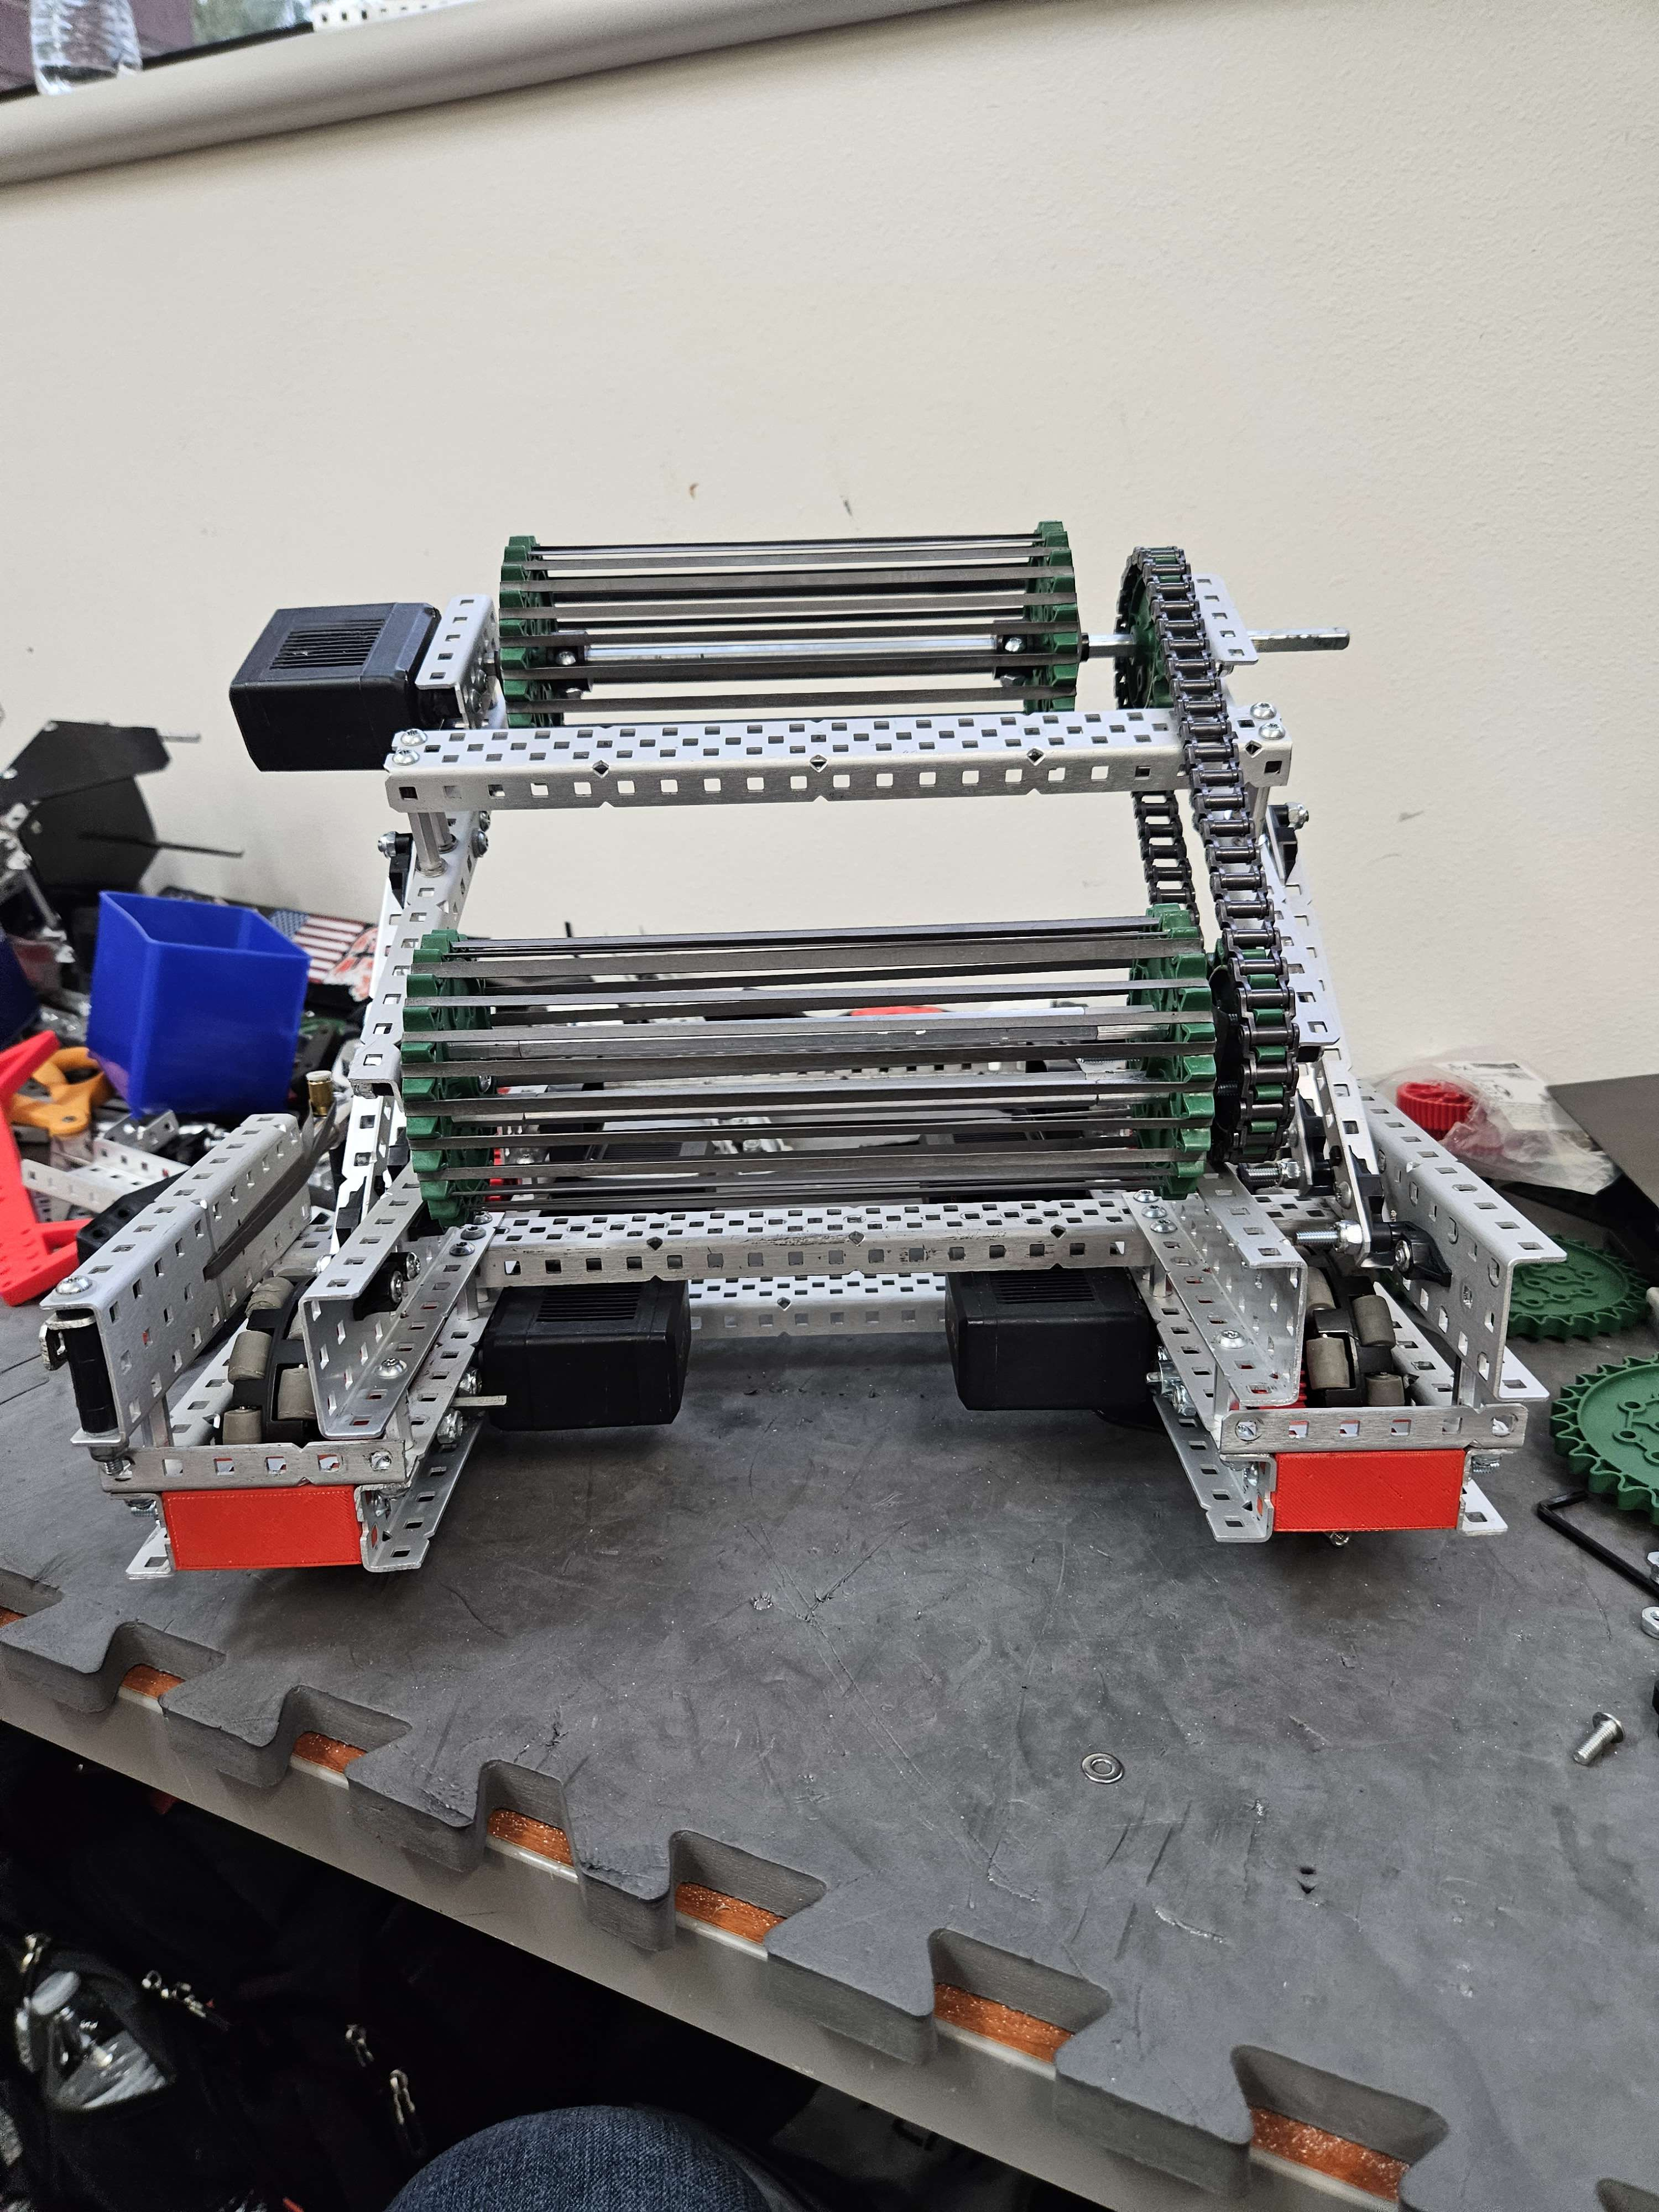
\includegraphics[width=0.5\linewidth]{images/october/first iteration of intake.jpg}
    \caption{Just a test}
    \label{fig:first iteration of intake}
\end{figure}

\section{2/19/2024}
Braden had a last ditch effort at getting RAMSETE to work before moving on to
tuning the PID constants for point-to-point movements and turns. While Braden
and Darrius were tuning the PID constants, an issue was discovered with the
pointTorward movement where turning to \degree{0} from \degree{180} would result
in no movement. This was rectified by testing the same code by itself and
adjusting how we offset the value from arctan to fit the field. Darrius took the
translated points from yesterday and converted them into proper C++ methods in
the 24" and 15" robot classes. Darrius also hooked up the LVGL autonomous
selector with the rest of the program and tested that the corresponding routine
and color values changed.
\section{2/20/2024}
Braden continued tuning the PID values for the autonomous routines, before
beginning work on the autonomous routines. Starting from what Darrius had,
Braden tuned the 24" while Darrius worked with the 15". During testing, it was
discovered a wire for an odometer on the 15" had gone bad. Additionally, the GPS
sensors were returning NaN values (not-a-number) and were generally noisy and
unreliable, so they were removed for the time being. This poses a significant
issue during autonomous because the GPS was the only sensor we had that could
detect side-to-side movement. The error brought by this loss can be somewhat
mitigated by avoiding significant collisions where we "slide" (and thus move to
our side).
\section{2/21/2024}
Braden discovered that there was no issue with the robot reversing, but rather
the value for motor voltage had accidentally been placed where the "reversed"
boolean parameter goes and was automatically coerced into a boolean value. When
this was corrected, the issue was resolved. Braden continued testing the match
autonomous and decided to add additional factories for different PID values for
if the robot was going a long or short distance. After these changes, the
autonomous routines for the 24" and 15" were nearly done, although the 15" had
to be adjusted to be in time. Everett pointed out that sleds on the 24" went
within the blue goal while scoring and was, therefore, technically illegal. This
was rectified by adding a simple spacer to the back of the robot.
\section{2/22/2024}
Braden adjusted the timing for the 15" and now both robots are both within 45
seconds and getting the win point. Braden then worked on the autonomous skills
for both robots. Since match loading and shoving the triballs is a large portion
of the routine, once the 24" routine was complete, the 15" routine followed suit
quickly. Darrius made some last minute changes to the GUI while helping with
setting up for the skills routines with Everett and Preston. Finally, Braden
adjusted some code to make it easier to read for the sake of the judges at
Houston.